\documentclass[10pt, a4paper]{article}

\usepackage[a4paper, margin=2.5cm]{geometry}
\usepackage{listings}
\usepackage{xcolor}
\usepackage{hyperref}
\usepackage{titlesec}
\usepackage{fancyhdr}
\usepackage{booktabs}
\usepackage{array}
\usepackage{amsmath}
\usepackage{parskip}
\usepackage{enumitem}
\usepackage{microtype}
\usepackage{fontenc}
\usepackage{inputenc}
\usepackage{tikz}
\usetikzlibrary{positioning}
\usepackage{mdframed}

% Colors
\definecolor{codebg}{HTML}{F5F5F5}
\definecolor{codeframe}{HTML}{CCCCCC}
\definecolor{codegreen}{HTML}{008000}
\definecolor{codegray}{HTML}{555555}
\definecolor{codeblue}{HTML}{0000FF}
\definecolor{codered}{HTML}{A31515}
\definecolor{linkblue}{HTML}{0563C1}
\definecolor{notebg}{HTML}{EFF6FF}
\definecolor{noteframe}{HTML}{3B82F6}
\definecolor{warnbg}{HTML}{FFFBEB}
\definecolor{warnframe}{HTML}{F59E0B}

% Hyperref
\hypersetup{
    pdftitle   = {Uploading Code to Arduino Using ESP-32 Wirelessly},
}

% Code style
\lstdefinestyle{codestyle}{
    backgroundcolor = \color{codebg},
    basicstyle      = \ttfamily\small,
    keywordstyle    = \color{codeblue}\bfseries,
    commentstyle    = \color{codegreen}\itshape,
    stringstyle     = \color{codered},
    breaklines      = true,
    keepspaces      = true,
    showstringspaces= false,
    frame           = single,
    framerule       = 0.4pt,
    rulecolor       = \color{codeframe},
    xleftmargin     = 6pt,
    xrightmargin    = 6pt,
    aboveskip       = 6pt,
    belowskip       = 6pt,
    tabsize         = 2,
}
\lstset{style=codestyle}

% Section styles
\titleformat{\section}{\large\bfseries}{\thesection.}{0.5em}{}
\titleformat{\subsection}{\normalsize\bfseries}{\thesubsection}{0.5em}{}
\titleformat{\subsubsection}{\normalsize\itshape}{}{}{}

% Header/Footer
\pagestyle{fancy}
\fancyhf{}
\fancyhead[L]{\small Uploading Code to Arduino Using ESP-32 Wirelessly}
\fancyhead[R]{\small Scientific Programming}
\fancyfoot[C]{\thepage}
\renewcommand{\headrulewidth}{0.4pt}

% Note boxes
\newmdenv[
    backgroundcolor=notebg, linecolor=noteframe, linewidth=1.5pt,
    leftline=true, rightline=false, topline=false, bottomline=false,
    innerleftmargin=10pt, innerrightmargin=8pt,
    innertopmargin=6pt, innerbottommargin=6pt,
    skipabove=6pt, skipbelow=6pt,
]{notebox}

\newmdenv[
    backgroundcolor=warnbg, linecolor=warnframe, linewidth=1.5pt,
    leftline=true, rightline=false, topline=false, bottomline=false,
    innerleftmargin=10pt, innerrightmargin=8pt,
    innertopmargin=6pt, innerbottommargin=6pt,
    skipabove=6pt, skipbelow=6pt,
]{warnbox}

\newcommand{\ic}[1]{\texttt{\small #1}}

\begin{document}

% Title
\title{\textbf{Uploading Code to Arduino Using ESP-32 Wirelessly}}
\author{Darsh Gajare - EE25BTECH11020 \\ Nishid Khandagre - EE25BTECH11043}
{\let\newpage\relax\maketitle}
\tableofcontents

% I. Introduction
\section{Introduction}

Uploading code to an Arduino through a phone can be done using applications
like ArduinoDroid; however uploading solely through Termux is different because
Termux does not have permission to directly access the USB port on Android devices.

This document describes a hardware workaround: an ESP32 acts as a
transparent bridge between WiFi and UART, forwarding the STK500 programming
protocol from the phone to the Arduino bootloader wirelessly.

\section{Overview}

\begin{center}
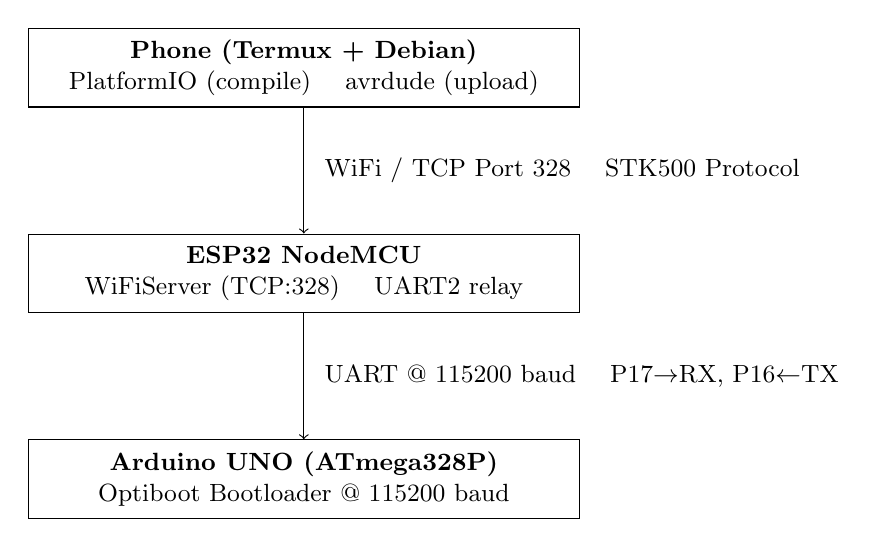
\begin{tikzpicture}[
    box/.style={draw, rectangle, minimum width=7cm, minimum height=1cm,
                align=center, font=\small},
    node distance=1.6cm
]
    \node[box] (phone)
        {\textbf{Phone (Termux + Debian)}\\
         \small PlatformIO (compile) \quad avrdude (upload)};

    \node[box, below=of phone] (esp)
        {\textbf{ESP32 NodeMCU}\\
         \small WiFiServer (TCP:328) \quad UART2 relay};

    \node[box, below=of esp] (uno)
        {\textbf{Arduino UNO (ATmega328P)}\\
         \small Optiboot Bootloader @ 115200 baud};

    \draw[->] (phone.south) -- node[right, font=\small, xshift=4pt]
        {WiFi / TCP Port 328 \quad STK500 Protocol} (esp.north);
    \draw[->] (esp.south) -- node[right, font=\small, xshift=4pt]
        {UART @ 115200 baud \quad P17$\to$RX, P16$\leftarrow$TX} (uno.north);
\end{tikzpicture}
\end{center}

The phone compiles the sketch using PlatformIO and invokes \ic{avrdude}, which
opens a TCP socket to the ESP32 on port 328. The ESP32 forwards all bytes
transparently between the socket and UART2, relaying the STK500 protocol to the
Arduino bootloader.

\section{Hardware Connections}

\subsection{Pin Wiring}

\begin{center}
\begin{tabular}{llll}
\toprule
\textbf{ESP32 Pin} & \textbf{Arduino Pin} & \textbf{Dir.} & \textbf{Note} \\
\midrule
5V        & VIN        & $\to$             & Power via onboard regulator \\
GND       & GND        & $\leftrightarrow$ & Common ground --- essential \\
P17 (TX2) & Pin 0 (RX) & $\to$             & Direct wire \\
P16 (RX2) & Pin 1 (TX) & $\leftarrow$      & Via 3$\times$10k$\Omega$ voltage divider \\
P4        & RST        & $\to$             & Reset control \\
\bottomrule
\end{tabular}
\end{center}

\subsection{Voltage Divider}

Arduino TX outputs 5V logic. The ESP32 GPIO pins supports 3.3V.
A resistor voltage divider on the P16 (RX2) line is required:

\[
V_{out} = V_{in} \times \frac{R_2}{R_1 + R_2}
        = 5\,\text{V} \times \frac{10\,\text{k}}{30\,\text{k}}
        = 3.3\,\text{V}
\]

\subsection{Reset Capacitor}

A 100~$\mu$F electrolytic capacitor connected between Arduino RST (+) and
GND ($-$) extends the bootloader window to 1--3~seconds, giving us time to press reset button on Arduino.

\section{ESP32 Firmware flashing using ArduinoDroid}

The ESP32 firmware starts a TCP server on port 328 and relays bytes between
the WiFi socket and UART2.Code for ESP32:
\begin{notebox}
\href{https://github.com/gajaredarsh/esp-flasher/blob/main/esp_programmer/main.ino}{\ic{esp32\_programmer/main.ino}}.
\end{notebox}
Replace \ic{YOUR\_SSID} \& \ic{YOUR\_PASSWORD} with the SSID and Password of the network you are using.\\
\begin{enumerate}[leftmargin=*, itemsep=2pt]
    \item Install \textbf{ArduinoDroid} from the Play Store
    \item Connect ESP32 to phone via OTG cable
    \item Open ArduinoDroid $\to$ paste firmware $\to$ select \textbf{ESP32 Dev Module}
    \item Tap \textbf{Upload} (hold BOOT on ESP32 if upload fails)
    \item Use Serial Monitor at 115200~baud to read the IP address
\end{enumerate}

% VI. Arduino Project
\section{Arduino Project Setup}

\subsection{Create Project}

\begin{lstlisting}[language=bash, caption={Initialize Arduino project}]
mkdir arduino_code && cd arduino_code
pio init --board uno
nvim src/main.cpp    # write your sketch
\end{lstlisting}

\subsection{PlatformIO Configuration}
Paste this code in platformio.ini
\begin{notebox}
\href{https://github.com/gajaredarsh/esp-flasher/blob/main/arduino-code/platformio.ini}{\ic{arduino\_code/platformio.ini}}.
\end{notebox}
Replace \ic{ESP\_IP} with your ESP32's IP address (e.g.\ \ic{192.168.43.100}).

% VII. Uploading
\section{Uploading Firmware Wirelessly}

\begin{lstlisting}[language=bash, caption={Build and upload}]
cd arduino_code
pio run --target upload
\end{lstlisting}

Press RST on the Arduino immediately after running the command.

% VIII. Finding IP
\section{Finding the ESP32 IP Address}

The ESP32 IP address changes when switching networks. Method to find it: \\
\textbf{ArduinoDroid Serial Monitor} --- connect via OTG, open Serial
          Monitor at 115200~baud, press RST on ESP32


% IX. Timing Issue
\section{The Timing Issue}

Uploading relies on the Arduino auto-reset mechanism. When a serial connection
opens, the DTR line drops, pulsing the RESET pin and forcing the Arduino into
bootloader mode. The bootloader listens for only $\approx$1~second before timing out.

Over TCP, avrdude cannot control DTR automatically. The 100~$\mu$F capacitor
(Section~3.3) solves this by extending the window to 1--3~seconds.


\end{document}
